%==========================================================================

\begin{frame}[fragile]

  {\Huge Backend Updates}

  \vspace{10pt}

\end{frame}

%==========================================================================

\begin{frame}[fragile]

  {\Huge CUDA}

  \vspace{10pt}

\end{frame}

%==========================================================================

\begin{frame}[fragile]{128 Bit CAS-based device atomics on Hopper and Blackwell (CUDA $>=$ 12.8)}

\begin{figure}[ht]
\centering
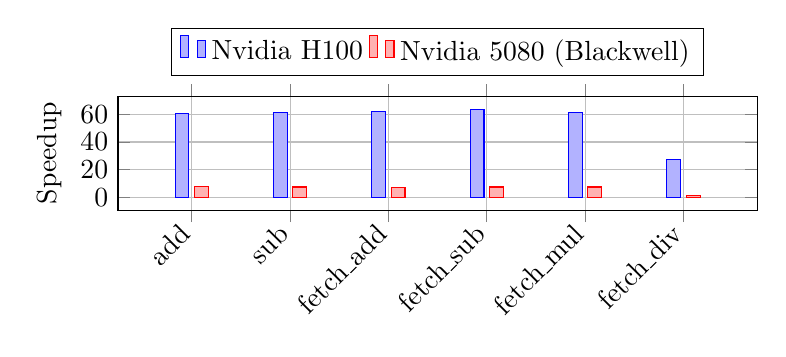
\begin{tikzpicture}
\begin{axis}[
    %title={Atomics on $10^8$\texttt{Kokkos::complex<double>} \textbf{without} contention},
    width=0.8\textwidth,
    height=0.25\textwidth,
    grid=major,
    ymin=0,
    ybar,
    ybar=2pt,
    bar width=5pt,
    enlargelimits=0.15,
    legend style={at={(0.5,1.6)},
      anchor=north,legend columns=-1},
    ylabel={Speedup},
    symbolic x coords={add,sub,fetch\_add,fetch\_sub,fetch\_mul,fetch\_div},
    xtick=data,
    x tick label style={rotate=45,anchor=east},
    %nodes near coords,
    %nodes near coords align={vertical},
    ]
\addplot coordinates {(add,60.9383491542) (sub,61.3601695793) (fetch\_add,62.2689318092) (fetch\_sub,63.6933886833) (fetch\_mul,61.4623888556) (fetch\_div,27.1370696705)};
\addplot coordinates {(add,7.5113136277) (sub,7.3840995425) (fetch\_add,7.2957874994) (fetch\_sub,7.3351913106) (fetch\_mul,7.3557821451) (fetch\_div,1.2353750828)};
\legend{Nvidia H100, Nvidia 5080 (Blackwell)}
\end{axis}
\end{tikzpicture}
\end{figure}
\begin{itemize}
  \item Atomics on $10^8$\texttt{Kokkos::complex<double>} \textbf{without} contention
\begin{itemize}
    \item Speedup $\approx 60x$ on H100 and $\approx 7$ on RTX5080.
    \item Same performance for \texttt{int128} and \texttt{Kokkos::complex<double>}.
    \item Division more costly, thus less effect of atomic CAS.
\end{itemize}
\end{itemize}

\end{frame}

%==========================================================================

\begin{frame}[fragile]{Effect of contention on \texttt{atomic\_add} on Hopper}

\begin{figure}[ht]
\centering
  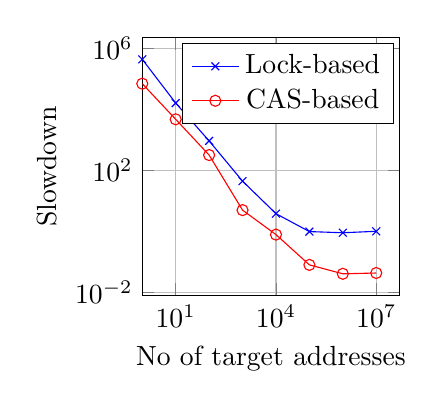
\begin{tikzpicture}
    \begin{loglogaxis}[
    %title={\texttt{atomic\_add} of \texttt{Kokkos::complex<double>} with $10^8$ workers},
    width=0.4\textwidth,
    height=0.4\textwidth,
    log basis x = 10,
    grid=major,
    xmin=1,
    xlabel={No of target addresses},
    ylabel={Slowdown}
    ]
    \addplot+[mark=x] coordinates {
		(1,430493.9171899781)
		(10,15898.3990852844)
		(100,915.3459702246)
		(1000,43.9645742601)
		(10000,3.777034824)
		(100000,0.9787170675)
		(1000000,0.8960538272)
        (10000000,1.0)
        };
    \addplot+[mark=o] coordinates {
		(1,68593.7222119811)
		(10,4665.2018278071)
		(100,314.4430296381)
		(1000,4.9384166747)
		(10000,0.7793873907)
		(100000,0.07931081247)
		(1000000,0.04049346243)
        (10000000,0.04297514822)
        };
    \legend{Lock-based,CAS-based}
    \end{loglogaxis}
  \end{tikzpicture}
  \caption{\texttt{atomic\_add} of \texttt{Kokkos::complex<double>} with $10^8$ workers}
\end{figure}
  \vspace{-0.8cm}
\begin{itemize}
    \item Effectiveness of CAS-based atomics reduces similar to Lock-based atomics at high contention.
\end{itemize}

\end{frame}


\begin{frame}[fragile]{Use up to 32kb of constant memory on CUDA}

\begin{itemize}
    \item Allows to launch kernels with up to 32kb of arguments in constant memory. Previously it was 4kb.
    \item Effect visible for functors that use data in the 4kb to 32kb range. No effect on smaller or larger functors.
    \item This can change the synchronization behavior for functors in this range as it reduces launch latency and runtime.
    \item Only working with \texttt{nvcc} $>=12.2$ and $>=$ Volta.
\end{itemize}

\end{frame}

%==========================================================================

\begin{frame}[fragile]

  {\Huge SYCL and OpenMPTarget}

  \vspace{10pt}

\end{frame}

%==========================================================================

\begin{frame}[fragile]{Use unsigned integer type as \texttt{size\_type} in SYCL}

\begin{itemize}
  \item \texttt{SYCL} now uses an unsigned integer type as \texttt{size\_type}.
    \item Now unsigned integer type across all backends.
\end{itemize}

\end{frame}

%==========================================================================

\begin{frame}[fragile]{Allow \texttt{parallel\_scan} to start anywere in OpenMPTarget}

\begin{itemize}
  \item Previously \texttt{parallel\_scan} with a \texttt{RangePolicy} needed to start at index 0
  \item Now any starting at index smaller than the end index is supported.
\end{itemize}

\end{frame}

%==========================================================================
